\documentclass[twoside,twocolumn,11pt]{article}
\batchmode
\linespread{2} 
\usepackage[english]{babel} 
\usepackage{natbib}
\usepackage[switch]{lineno} 
\usepackage[hmarginratio=1:1,top=32mm,columnsep=20pt]{geometry} 
\usepackage[hang, small,labelfont=bf,up,textfont=it,up]{caption} 
\usepackage{booktabs} 
\usepackage{graphicx}
\usepackage{microtype}
\usepackage{caption}
\graphicspath{ {../Data/} } \usepackage{caption}
\usepackage{lettrine} 
\usepackage{csvsimple}
\usepackage{tabulary}
\usepackage{enumitem} 
\setlist[itemize]{noitemsep} 
\usepackage{abstract} 
\renewcommand{\abstractnamefont}{\normalfont\bfseries} 
\renewcommand{\abstracttextfont}{\normalfont\small\itshape} 

\usepackage{titlesec} 
\renewcommand\thesection{\Roman{section}} 
\renewcommand\thesubsection{\roman{subsection}} 
\titleformat{\section}[block]{\large\scshape\centering\bfseries}{\thesection.}{1em}{} 
\titleformat{\subsection}[block]{\large\bfseries}{\thesubsection.}{1em}{}

\usepackage{titling} 

\setlength{\droptitle}{-4\baselineskip} 

\pretitle{\begin{center}\Huge\bfseries} 
\posttitle{\end{center}} 
\title{Modelling Thermal Responses of Metabolic Traits} 
\author{ \\
\textsc{Jacob Griffiths} \\
\normalsize Imperial College London \\ 
\normalsize jacob.griffiths18@imperial.ac.uk \\
\normalsize Word count: 2992
}
\date{March 8, 2019} 
\renewcommand{\maketitlehookd}{


}


\begin{document}


\twocolumn[{%
\renewcommand\twocolumn[1][]{#1}%
\maketitle
\begin{center}
    \centering
    \includegraphics[width=.50\textwidth,height=8.5cm]{imperial.png}
\end{center}%
}]


\clearpage

\linenumbers

\twocolumn[
  \begin{@twocolumnfalse}
    \begin{abstract}
      Temperature is the one of the most important factors in determining metabolic rate and 
      the optimisation of metabolic rate will tend to increase the fitness of any organism. 
      Climate change is already having an enourmous impact on all life on Earth and ectotherms
      can be particularly sensitive to environmental shifts in temperature. Many species are
      resorting to latitudinal range shifts, as well as behavioural and evolutionary adaptation, 
      but extinction is often unavoidable. Improving our ability to model thermal responses is 
      vital if we are to predict, understand, and hopefully prevent, future extinctions.
      This study compared the relative ability of three models, the cubic polynomial, Briere, and
      Schoolfield, each being fitted to 1367 datasets within the BioTraits meta-dataset. It was concluded
      that the Briere model was the best based on these data, affirmed by consistently better 
      $AIC_c$ scores. \\
    \end{abstract}
  \end{@twocolumnfalse}
]


\section{Introduction}

Temperature is a fundamental parameter in
almost all biological processes and its importance in metabolic biology is well 
documented \citep{Brown2004, Montoya2012, Dell2011,DeLong2017}. 
Metabolic processes are often catalysed by enzymes
which depend on kinetic, and ultimately heat, energy to function. As temperature
decreases, molecules have less and less kinetic energy, decreasing the acquisition rate of 
substrate by enzyme units, and thus metabolic rates
decrease accordingly. When temperature increases, metabolic rates increase steadily
until the thermal optimum is reached  \citep{DeLong2017, Dell2011}; that is, the temperature at which optimal
metabolic rate occurs ($T_{pk}$ or $T_{opt}$). Beyond this, increasing temperature
will start to hinder the metabolic rate until the lethal limit is reached. The mechanisms
behind this sharp decline in metabolic rate are disputed but could potentially be
due to protein degradation \citep{Johnson1946, Dell2011}. These metabolic responses 
to temperature exhibit a remarkably similar pattern graphically, often referred to as Thermal 
Performance Curves (TPCs), across a plethora of metabolic processes and taxa. This 
makes the study of TPCs a useful tool of comparison for all life on Earth as all
living things depend on metabolism for their energy. Furthermore, an increased understanding
of how species respond to temperature is imperative in a rapidly warming world. 
If we can find some plasticity in a species' temperature tolerance then perhaps it will
have a better chance of avoiding the mass extinction that is sweeping our planet,
although some recent findings suggest the scope for adaptation may be limited \citep{Tuzun2018}.
Of course, there are other ways a species may adapt, for example through latitudinal range shifting \citep{Haase2019}
or evolution. However, the latter seems unlikely in the time-frame available, although some 
studies have suggested it is possible \citep{DeLong2018}, and the former
is only possible for mobile species with suitable habitats to move to.
The database used in this study, BioTraits, was provided by my supervisor,
Dr. Samraat Pawar, and is an extension of the database used by \cite{Dell2011} and \cite{Kontopoulos2018}. It 
is one of the most extensive metabolic datasets ever amalgamated and provided an excellent
way to compare three different models for TPCs.

\subsection{Models}
Three models were used in this study to compare their ability to fit to each dataset within BioTraits.
Firstly, there is the phenomenological cubic polynomial:
\begin{equation}
B = B_0 + B_1T + B_2T^2 + B_3T^3
\end{equation}
Where $B$ is the responding trait value, $T$ is the temperature, $B_0$ is the $y$-intercept of the 
curve, and $B_1$, $B_2$, and $B_3$ are coefficients acting on $T$.

Secondly, the Briere model \citep{Briere1999} was used as an alternative phenomenological model:
\begin{equation}
  B = B_0T(T - T_{0})\sqrt{T_{m} - T}
\end{equation}
Where $T_{0}$ and $T_{m}$ are the minimum and maximum thermal tolerances respectively for the trait - $B$ - and $B_0$ 
is a normalisation constant. Whilst this model is technically phenomenological, it can still provide useful 
biological insight once fitted as it gives an estimate of the thermal
tolerance of a particular trait for a particular organism; as it has $x$-intercepts ($T$), and its parameters meet the definition of `ecological
parameters' coined by \citep{Lamb1984}. However, it falls short of the definition
of a mechanistic model as the model provides no insight into the underlying biological mechanisms at work.

Finally, the third model used in this study was a simplified version of the Sharpe-Schoolfield \citep{Schoolfield1981}
model to provide a mechanistic comparison as it is derived from thermodynamic and enzyme 
kinetic theory. The full model is given by:
\begin{equation}
  B = \frac{B_{0}e^{\frac{-E}{k}(\frac{1}{T} - \frac{1}{283.15})}}{1 + e^{\frac{E_l}{k}(\frac{1}{T_l} - \frac{1}{T})} + e^{\frac{E_h}{k}(\frac{1}{T_h} - \frac{1}{T})}}
\end{equation}
Where $k$ is the Boltzmann constant ($8.617 \times 10^{-5}  \ $eV$ \ \dot K^{-1}$, \cite{Boltzmann1872}), 
T is the temperature in Kelvin, $B_0$ is the trait value at a reference temperature - 283.15 K in this study - 
$E_l$ is the low-temperature deactivation energy (eV) of the enzyme 
and controls the behaviour of the curve at very low temperatures and $T_l$ is the temperature at which 50\% of 
enzyme units have been low-temperature deactivated. $E_h$ is the high-temperature deactivation energy of the enzyme and controls 
the behaviour of the curve beyond $T_{pk}$, and $T_h$ is the temperature at which 50\% of enzyme units have been
high-temperature deactivated. $E$ is the activation energy which controls the behaviour of the curve in the enzyme's 
'normal operating range', that is, before $T_{pk}$ but not at low temperatures.
This model attempts to capture the 
non-linear rate acceleration ($E_l$) at low temperatures, the linear rate increase, $E$, up to $T_pk$, and rapid non-linear 
deceleration, $E_h$, at high temperatures as the temperature approaches the lethal limit of an enzyme. This makes the
Briere model an interesting comparison as this too attempts to capture the two non-linear and linear aspects
of a typical TPC. There are also two simplified versions of the Schoolfield model, each with either the $E_h$ or $E_l$ 
element removed from the denominator. The removal of $E_l$ and associated terms is sometimes intuitive as 
low-temperature deactivation of enzymes is weak
and there is often insufficient data at low temperatures, as is the case with BioTraits. For these reasons, this simplified 
version was used for this study and is given by:
\begin{equation}
  B = \frac{B_{0}e^{\frac{-E}{k}(\frac{1}{T} - \frac{1}{283.15})}}{1 + e^{\frac{E_h}{k}(\frac{1}{T_h} - \frac{1}{T})}}
\end{equation}
Simplifying the model also allows for more datasets to be explained as the minimum number of datapoints required for the 
six-parameter model would be larger than for the four-parameter simplified version. Other studies, such as \cite{Alber1993}, 
have demonstrated that the simplified Schoolfield models often fit better. The reference temperature for this study
was set at 283.15 K as it has proved a reliable reference in other studies of this nature \citep{Dell2011} 
and seems more appropriate for the many cold-adapted species represented in BioTraits, despite 
\cite{Schoolfield1981} using a reference of 298.15 K. Assuming there has been no low- or high-temperature deactivation 
$B_0$ can be used as an approximation of the trait value at this reference temperature.
This study will be based on comparisons of these models, in the vein of
\cite{Johnson2004}, as opposed to traditional null-hypothesis testing,
as they demonstrated the power of model comparison with large sets of observational data.


\section{Methods}

\subsection{Computing Languages}
\subsubsection{R}
R (3.2.3) is a popular programming language within the biological sciences and is particularly powerful for statistical
analysis, data manipulation, and data visualisation \citep{R2015}. RStudio (1.1.419) was used as an interactive 
development environment (IDE) for R in this study as it 
permits the display of graphics and code within the same pane which is useful for visualisation \citep{RStudio2016}.
R was predominantly used in this study to 'wrangle' BioTraits, that is, to prepare
a filtered version for model fitting. It was then used post-fitting to visualise the models with optimised parameters, in
particular making use of the package ggplot2 (3.1.0) \citep{ggplot22016} to create aesthetic and intuitive plots.

\subsubsection{Python}
Python (3.5.2) is an immensely popular, object-oriented programming language first developed by \cite{Python1991}. It can lend 
its popularity, in part, to its extensive collection of packages, as well as its intuitive syntax,
making it one of the most versatile programming langauges.
In particular, the package lmfit \citep{lmfit2014} has robust functions for optimising model parameters using non-linear 
least-squares techniques which were used to fit the models in this study. Furthermore, Python is relatively fast, computationally 
speaking, at looping,
which gives it further advantage over R for fitting models to large datasets like BioTraits. Visual Studio Code \citep{VSCode2019} 
was used as an IDE for Python and IPython \citep{IPython2007} was used as a command shell for testing code as it has 
particularly good debugging features.

\subsubsection{Bash}
Bash (4.3.48) is an open-source, UNIX shell and command language originally created by \cite{Fox1989}. It is the default 
shell language used for most Linux distributions such as Ubuntu 16.04 which was the operating system used in this study. 
A Bash script was used to run each of the scripts used in this project as it is a versatile language that can easily 
call and run other languages.

\subsection{Data}
BioTraits consists of 2165 unique thermal responses of metabolic 
processes from 1010 publications. Predominantly, respiration, growth, and photosynthetic
rate are the metabolic process being measured against temperature. BioTraits includes species from many 
Phyla with diverse life histories, but a majority of representatives are terrestrial
species, Arthropods being particularly well-represented. 
As this dataset contains 155 columns and 25826 rows, it was first refined to a handful
of columns relevant to this study to improve computational speed, namely the trait value and temperature.
Rows with missing values for these columns were removed and any dataset with less than six unique
datapoints was also removed, as this is the minimum required to estimate four parameter models like the cubic
polynomial and simplified Schoolfield. 

\subsection{Parameter estimation}
Using R, starting parameters for every dataset in BioTraits were calculated.
For the cubic polynomial model, starting values of 1 were used for all four parameters.
For Briere, estimates for $T_{0}$ and $T_{m}$ were made using
the minimum and maximum observed temperatures respectively. For Schoolfield, a reference temperature of 283.15 K
was used and the parameter estimations were carried out following the method of
\cite{Schoolfield1981}. $B_{0}$ was estimated as the recorded trait value nearest to this temperature, as defined
by the equation. 
The peak metabolic 
rate $B_{max}$ was then calculated ($T_{pk}$ being the corresponding temperature at this trait value) and the dataset 
was split either side of this value. If $B_{max}$ occurred at the highest recorded temperature 
(i.e. the rate had not started descending yet) the dataset was not split and the subsequent regression was carried 
out on the whole dataset. The trait values were plotted on an Arrhenius plot ($log(trait)$ against $\frac{1}{kT}$) 
with $k$ being the Boltzmann constant. Linear 
regression was carried out on the left-hand (below $T_{pk}$) data and the estimate for $E$ was taken as the gradient
of this line, with the $Eh$ estimate being twice this value. If regression failed, default estimates of $0.65$ for $E$
and $1.3$ for $Eh$ were used as recommended defaults from the literature, and $E$ was given bounds of 0 to 3, while $Eh$ 
was bound between 0 and 6 to maintain theoretical accuracy 
\citep{Montoya2012, Dell2011, Allen2006}. $Th$ was estimated by calculating the nearest recorded 
temperature to $\frac{B_{max}}{2}$ as $Th$ is the temperature at which half the enzyme units have been made inactive, so this 
provides a good estimate, with a lower bound of $T_{pk}$ applied 
\citep{Kontopoulos2018}. For datasets with no datapoints after $B_{max}$, $Th$ was given a starting value equal to $T_{max}$. 

\subsection{Model comparison}
The Akaike Information Criterion ($AIC$) \citep{A1974} was used to compare model fits within each dataset and is 
given by the formula, assuming the model is univariate, is linear in its parameters, and has normally-distributed residuals:
\begin{equation}
  AIC = 2k - 2\ln(\hat{L})
\end{equation}
Where $\hat{L}$ is the maximum likelihood estimation of the model and $k$ is the number of parameters in the model.
$AIC$ rewards the relative goodness of fit between models applied to the same data but penalises 
number of parameters used as this can sometimes lead to overfitting.
This method was chosen over similar methods such as the Bayesian Information Criterion ($BIC$, \cite{Schwarz1978}) as it can be 
modified for small datasets and has higher success rates in picking the best model if the 'true' model is not
present in a sample of models \citep{Vrieze2012}. However, despite the existing penalty, $AIC$ can 
still be prone to favouring models with more parameters if the sample size is small (benchmark of at least 40
datapoints per model parameter suggested by \cite{Johnson2004}) and BioTraits includes several datasets that would
be susceptible to this. This can be circumvented by using $AIC_c$ \citep{Hurvich1989}, an extension of $AIC$ with
the addition of a further parameter penalty given by:
\begin{equation}
  AIC_c = AIC + \frac{2k^2 + 2k}{n-k-1}
\end{equation}
Where $n$ is the sample size and $k$ is the number of parameters as before. It should be noted that as $n \to \infty$, 
$\frac{2k^2 + 2k}{n-k-1} \to 0$ and thus $AIC_c \to AIC$, making it suitable for large samples too. 
As some of the datasets used in this analysis had only the minimum permittable number of datapoints to fit a four-
parameter model, $AIC_c$ was used to compare models instead of $AIC$.
\\
In addition to $AIC_c$, adjusted $R^2$, or $\bar{R}^2$, was used as an alternative comparison tool. Generally attributed 
to \cite{Wright1921}, $R^2$ is purely a measure of goodness of fit and is given by:
\begin{equation}
  R^2 = 1 - \frac{SS_{res}}{SS_{tot}}
\end{equation}
Where $SS_{res}$ is the sum of the squared residuals between the model and observed data and 
$SS_{tot}$ is the total sum of squares. A score 
of 1 is a 'perfect' fit and a negative score is considered a worse fit than a straight, horizontal line through the 
observed mean. $R^2$ is very susceptible to overfitting as the addition of a new parameter will always 
improve the score and this can lead to poor parameter estimatation which is particularly bad for model comparison
\citep{Johnson2004}. Fortunately, this can be accounted for to an extent with adjusted $R^2$, $\bar{R}^2$:
\begin{equation}
  \bar{R}^2 = 1 - (1-R^2) \frac{n-1}{n-k-1}
\end{equation}
Where $n$ is the number of datapoints and $k$ is the number of parameters. Unlike $R^2$, it only improves its 
score if an additional parameter improves the model more than would be expected by chance, making it less susceptible 
to overfitting and a better comparative tool for this study.


\section{Results}
Of the 2165 datasets in BioTraits, 1367 remained after the vetting criteria
was implemented. 
Starting parameters were then calculated for each dataset in R with varying success.
These parameters were then optimised in Python with no failed convergences (Table 1).
% latex table generated in R 3.2.3 by xtable 1.8-3 package
% Fri Mar  8 16:40:35 2019
\begin{table}[ht]
\centering
\caption{Median parameter estimates after optimisation} 
\scalebox{0.8}{
\begin{tabular}{rlll}
  \hline
 & Cubic & Briere & Schoolfield \\ 
  \hline
$B_0$ & 2340 & 0.0001434 & 1.271 \\ 
  $B_1$ & -23.62 & - & - \\ 
  $B_2$ & 0.08193 & - & - \\ 
  $B_3$ & -9.163e-05 & - & - \\ 
  $T_0$ & - & 277 & - \\ 
  $T_m$ & - & 318.5 & - \\ 
  $E$ & - & - & 0.6356 \\ 
  $E_h$ & - & - & 1.558 \\ 
  $T_h$ & - & - & 303.2 \\ 
   \hline
\end{tabular}
}
\end{table}

For Briere, the interquartile ranges of $B_0$, $T_0$ and $T_m$ were fairly narrow, as were 
the converged parameters for Schoolfield, although these were subject to far stricter bounds.
The datasets and associated optimised parameters were returned to R for visualisation and 
comparitive statistical analysis. An example plot is shown in Figure 1 and summarised $AIC_c$ and $\bar{R}^2$, 
values are shown in Table 2.
Mean $\bar{R}^2$ indicated that the cubic model had the best average fit, with Schoolfield second and
Briere last. Interestingly, Table 2 shows that despite this, if the best $\bar{R}^2$ counts are compared,
that is, the number of times each model had the highest $R^2$ value rather than the average,
cubic is still the best, but Briere replaces Schoolfield as second best.
With regards to $AIC_c$, Briere is considered the best model in the highest number of datasets, 
with cubic second best and Schoolfield worst.
% latex table generated in R 3.2.3 by xtable 1.8-3 package
% Fri Mar  8 16:40:35 2019
\begin{table}[ht]
\centering
\caption{Summary of comparative statistics for the three models.
                     The first and second rows are counts and the third row is the median adjusted $R^2$} 
\scalebox{0.8}{
\begin{tabular}{rlll}
  \hline
 & Cubic & Briere & Schoolfield \\ 
  \hline
Best $AIC_c$ & 372 & 549 & 203 \\ 
  Best adjusted $R^2$ & 708 & 336 & 306 \\ 
  Average adjusted $R^2$ & 0.8507 & 0.6655 & 0.7343 \\ 
   \hline
\end{tabular}
}
\end{table}



\begin{figure*}
  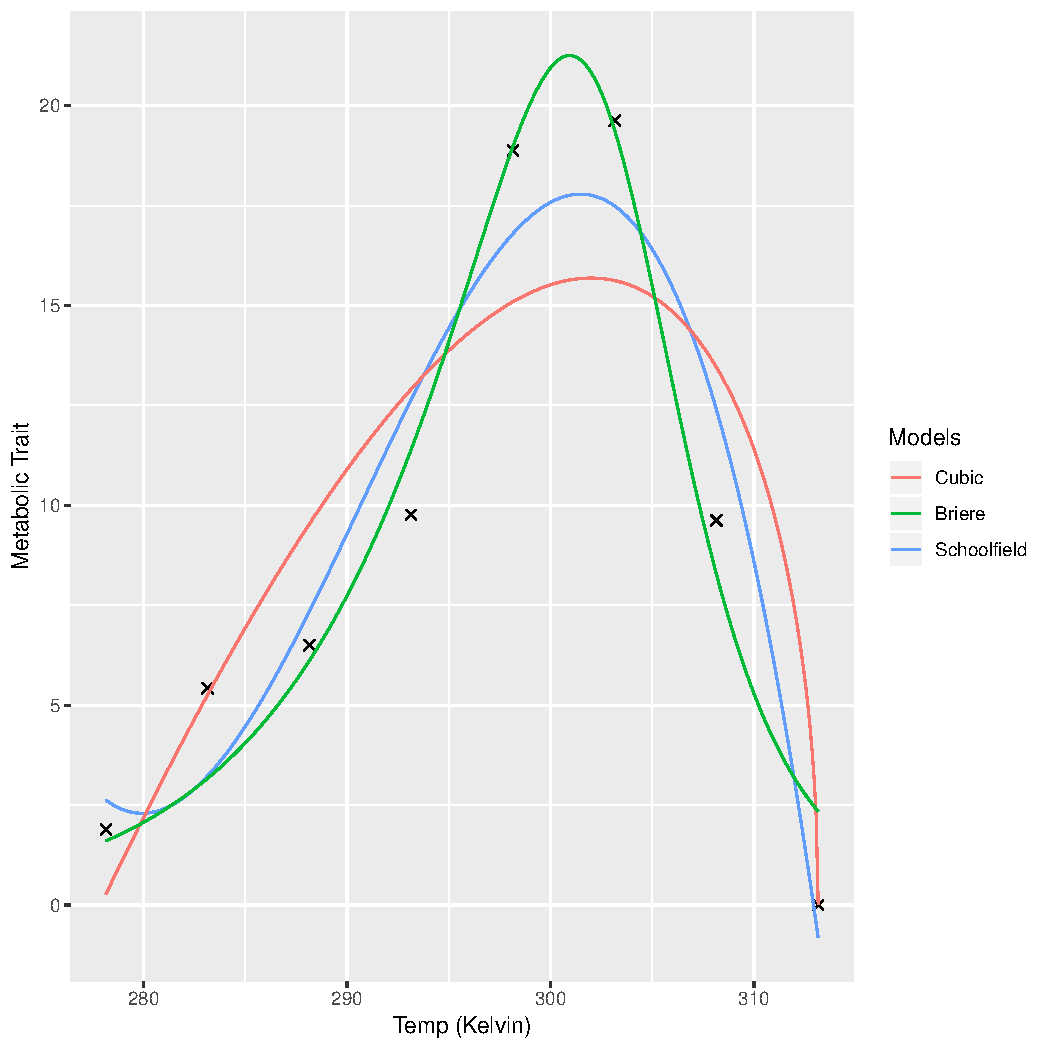
\includegraphics[width=\textwidth]{../Results/MTD2099.pdf}
  \caption{An example plot of the three models fitted to data used by
  \citep{Li2009}}
\end{figure*}



\section{Discussion}
For Schoolfield,
the regression carried out on the Arrenhius-transformed data was unreliable at providing 
'reasonable' starting estimates and defaults were often used as a result, as this provided
better fits in those cases. `Reasonable' estimates were defined as within or near the range established
by \cite{Dell2011}; for $E$ this was $0.2-1.2$. This may have been because a lot of the datasets used were quite small, and, after
being split about $B_{max}$, could lead to unrepresentative regression on the Arrhenius plots, leading to 
poor estimates for $E$ and
$E_h$. However, the apparent weakness in starting parameter estimation seemed to be mitigated
by the use of literature defaults as the average optimised parameters were similar to other studies 
\citep{Dell2011, Kontopoulos2018}. Average optimised parameters for $T_0$ and $T_m$ in the Briere model 
were slightly lower and higher respectively than the
estimates of \citep{Briere1999} ($T_0 = 283.15 K$, $T_m = 310.15 K$). This may be due to the larger and 
more taxonomically diverse nature of BioTraits as Briere's study was concerned exclusively 
with Arthropods. 

Comparing the models produced some conflicting but altogether more interesting results.
Cubic was the best fit according to the average $\bar{R}^2$ but this is not particularly
surprising when one considers the freedom with which its parameters can be varied without theoretical
and biological bounds. Of the other two models, Schoolfield had the higher average $\bar{R}^2$ but
Briere had a higher $\bar{R}^2$ in more datasets when count was considered, implying Briere had a 
greater range of fit consistency.
As the Briere model is based predominantly on the thermal responses of Arthropod metabolism, perhaps 
for these species it fit well and for other Phyla it was less competent.
Conversely, comparison through $AIC_c$ showed Briere to be the best model in the highest number 
of datasets, with cubic second and Schoolfield third. The discrepency between the two comparative
measures is intriguing and may be due to the additional parameter penalty that $AIC_c$ incorporates 
which would favour the Briere model over the other two as it requires one fewer parameter.
Moving forward, further research in this field would benefit by comparing more models, such as those proposed 
by \cite{DeLong2017}, and more data will undoubtedly improve reliability. Whilst BioTraits is one of the 
most extensive datasets
of its kind, it still shows clear bias towards certain Phyla, life histories, and climates, which will hinder
any extrapolations that can be drawn from models it fits well to.

In conclusion, the cubic model did fit well on average and was well-supported by $\bar{R}^2$, but the application 
of a purely phenomenological linear model to the proven non-linear response of metabolism to temperatures would limit any
useful biological interpretation and prediction going forward. The Schoolfield model has the advantage 
of parameters based on biological mechanisms but this study showed it was significantly less able to 
explain the data, particularly when $AIC_c$ was considered. Briere, however, proved to be the best model,
at least for BioTraits. It also has a distinct advantage over the cubic model in that, despite its lack
of mechanistic-underpinning, useful biological inferrences can be made when it is fit well. 

Ultimately, 
the 'best' model depends on the question you are asking. If the understanding of mechanism is your goal, Schoolfield
is still the best, as it is the only one of these three that is based on such theory. If you are interested 
in thermal tolerances, then the Briere model is a clear winner and if you wish only to identify an average response
for a particular organism or species then the cubic model is still a useful tool.

\cite{Levins1966} said that the unavoidable paradox of model fitting in biology is that one must sacrifice either 
generality, precision, or realism in the formulation of biological models.
Whilst many may dismiss the cubic model for its lack of mechanistic property, is 
sacrificing realism in using a phenomenological model like the cubic worse than sacrificing precision
by using a mechanistic model like Schoolfield? I would argue it is not.



Mention affect of bad B0 for schoolfield
Akaike weights and tings
Growth rate tends to have a non-linear relationship for arthropods \citep{Briere1999} which may make the cubic model 
less useful  for interpretation.
The Briere curve intercepts the temperature axis at high and low temperatures, allowing estimation 
of an upper and lower trait threshold.
AICc a much better comparison tool than $\bar{R}^2$ \citep{Johnson2004}
The cubic polynomial may have no biological underpinning but is sacrificing realism much different to 
sacrificing precision \citep{Levins1966}?


\bibliographystyle{agsm}
\bibliography{Miniproject}



\end{document}